\documentclass[12pt]{beamer}
\usepackage{pgf}
\usepackage[danish]{babel}
\usepackage[utf8]{inputenc}
\usepackage{beamerthemesplit}
\usepackage{graphics,epsfig, subfigure}
\usepackage{url}
\usepackage{srcltx}
\usepackage{hyperref}
\usepackage{fancybox}
\usepackage{listings}
\lstset{
  language=C,                % choose the language of the code
   basicstyle=\footnotesize,        % the size of the fonts that are used for the code
    keywordstyle=\color{blue},       % keyword style
     commentstyle=\color[rgb]{0.13,0.54,0.13},
  numbers=left,                   % where to put the line-numbers
  stepnumber= 0.3,                   % the step between two line-numbers.        
  numbersep=1pt,                  % how far the line-numbers are from the code
  backgroundcolor=\color{white},  % choose the background color. You must add \usepackage{color}
  showspaces=false,               % show spaces adding particular underscores
  showstringspaces=false,         % underline spaces within strings
  showtabs=false,                 % show tabs within strings adding particular underscores
  tabsize=2,                      % sets default tabsize to 2 spaces
  captionpos=b,                   % sets the caption-position to bottom
  breaklines=true,                % sets automatic line breaking
  breakatwhitespace=true,         % sets if automatic breaks should only happen at whitespace
 % title=\lstname,                 % show the filename of files included with \lstinputlisting;
}
\definecolor{kugreen}{RGB}{50,93,61}
\definecolor{kugreenlys}{RGB}{132,158,139}
\definecolor{kugreenlyslys}{RGB}{173,190,177}
\definecolor{kugreenlyslyslys}{RGB}{214,223,216}
\setbeamercovered{transparent}
\mode<presentation>
\usetheme[numbers,totalnumber,compress,sidebarshades]{PaloAlto}
\setbeamertemplate{section in toc}[sections numbered]

\setbeamertemplate{footline}[frame number]

  \usecolortheme[named=kugreen]{structure}
  \useinnertheme{circles}
  \usefonttheme[onlymath]{serif}
  \setbeamercovered{transparent}
  \setbeamertemplate{blocks}[rounded][shadow=true]

\logo{
\includegraphics[width=0.8cm]{fga_logo.png}}
%\useoutertheme{infolines} 
\title{Gestão de Portfólios e Projetos de Software}
\subtitle{Fases ou Grupos de Processo: Monitoramento e Controle}
\author{Dra. Carla Rocha, Msc. Hilmer R. Neri}


\institute{Engenharia de Software \\ Universidade de Brasília}
\date{2015.2}


\begin{document}
\frame{\titlepage \vspace{-0.5cm}	
}
\frame
{
\frametitle{Agenda}
\tableofcontents%[pausesection]
}
\section{Grupo de Processo Monitoramento e Controle}

\begin{frame}
 \frametitle{GRUPO DE PROCESSOS (“FASE”) – \small{EXECUÇÃO, MONITORAMENTO E ENCERRAMENTO}}
  \begin{figure}
   \centering
   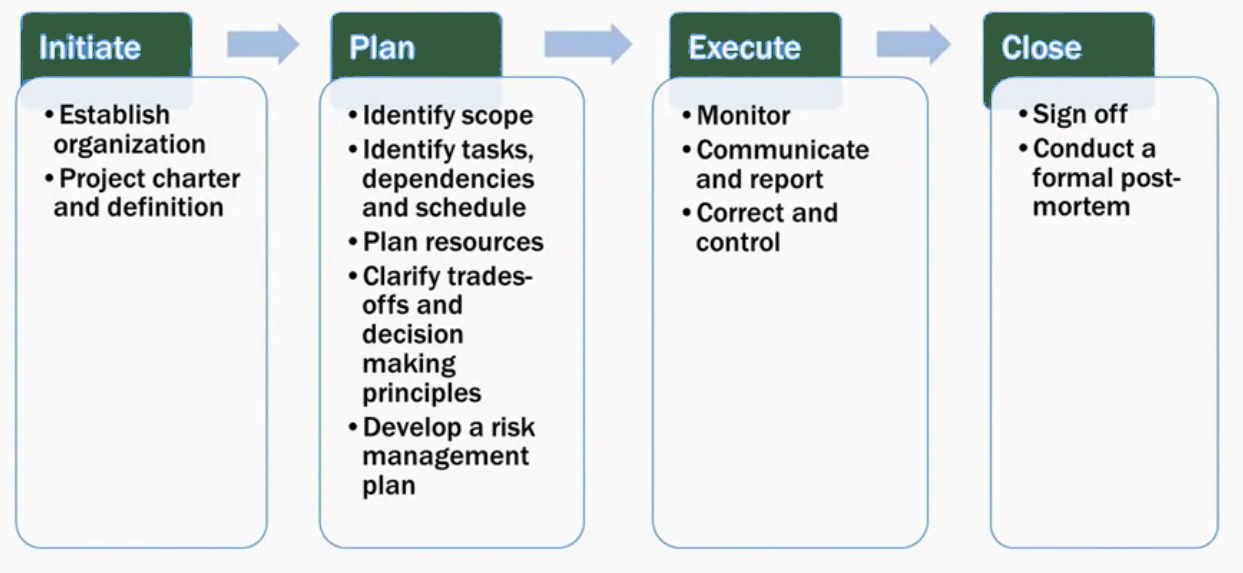
\includegraphics[width = 0.9\textwidth]{figs/fig0.png}
  \end{figure}
\end{frame}

\begin{frame}
 \frametitle{GRUPO DE PROCESSOS (“FASE”) – \small{EXECUÇÃO, MONITORAMENTO E ENCERRAMENTO}}
  \begin{figure}
   \centering
   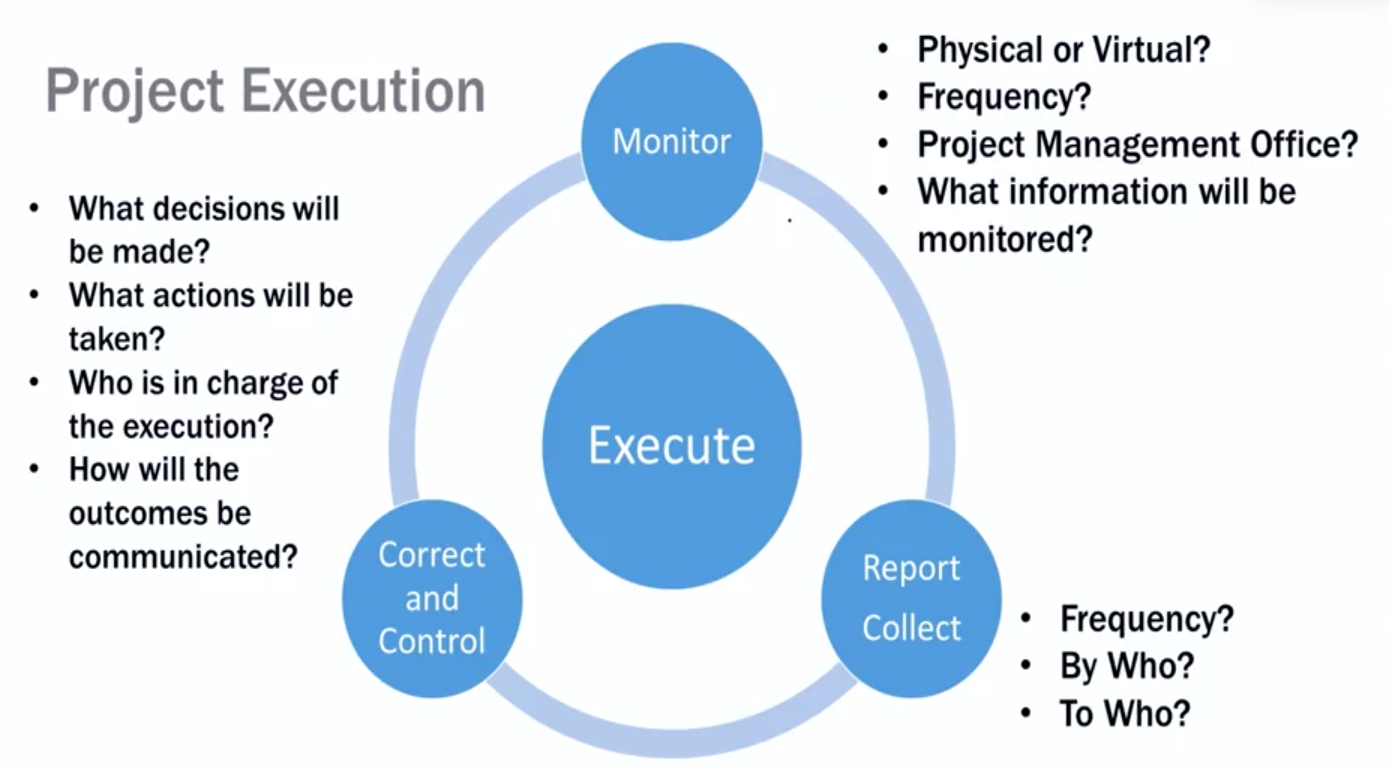
\includegraphics[width = 0.9\textwidth]{figs/fig11.png}
  \end{figure}
\end{frame}

\begin{frame}
 \frametitle{Relembrando - Planejamento do projeto "Startup"}
 Planejamento - Atividades, recursos, dependências
  \begin{figure}
   \centering
   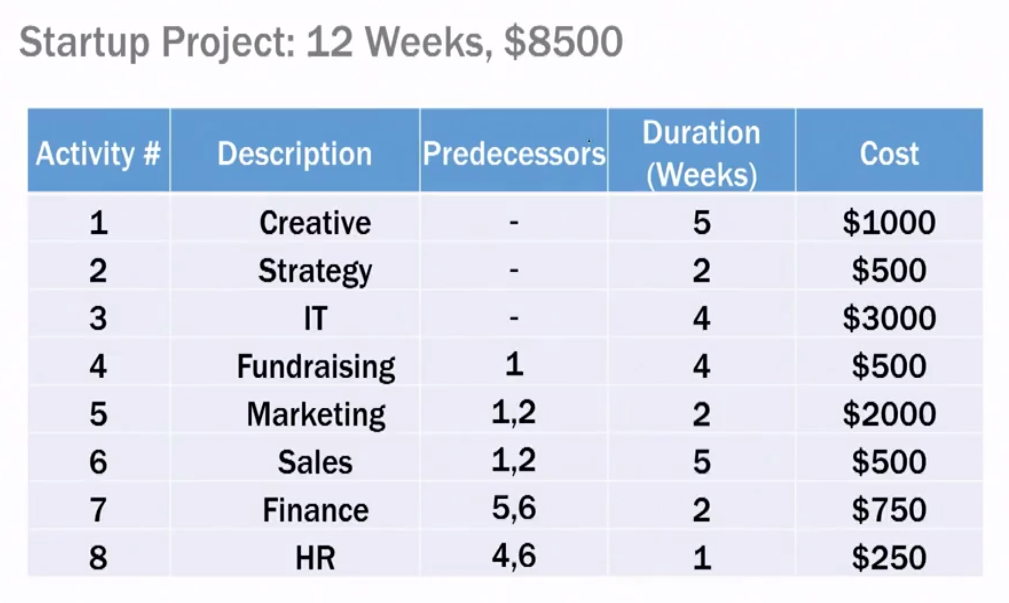
\includegraphics[width = 0.9\textwidth]{figs/fig12.png}
  \end{figure}
\end{frame}

\begin{frame}
 \frametitle{Relembrando - Planejamento do projeto "Startup"}
 Planejamento - Atividades, recursos, dependências
  \begin{figure}
   \centering
   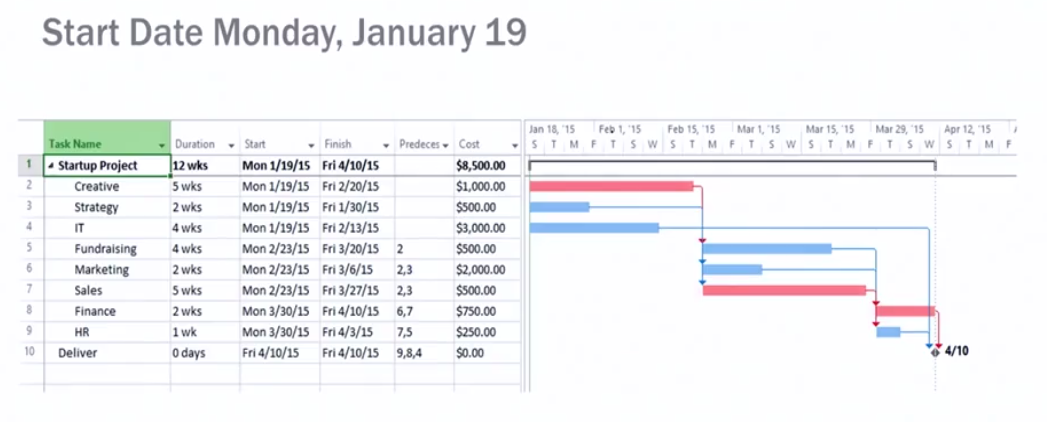
\includegraphics[width = 0.9\textwidth]{figs/fig13.png}
  \end{figure}
\end{frame}

\begin{frame}
 \frametitle{Relembrando - Planejamento do projeto "Startup"}
 Planejamento - Atividades, recursos, dependências
  \begin{figure}
   \centering
   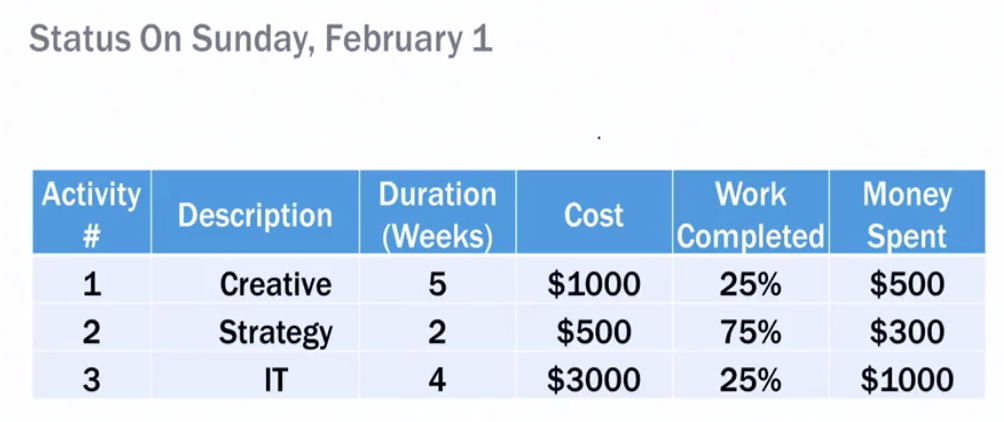
\includegraphics[width = 0.9\textwidth]{figs/fig14.png}
  \end{figure}
\end{frame}

\begin{frame}
 \frametitle{Relembrando - Planejamento do projeto "Startup"}
 Planejamento - Atividades, recursos, dependências
  \begin{figure}
   \centering
   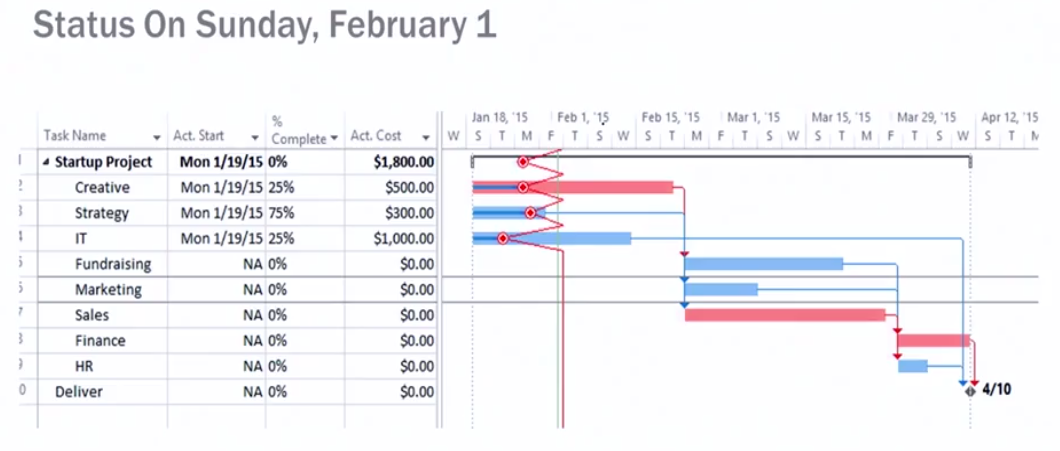
\includegraphics[width = 0.9\textwidth]{figs/fig15.png}
  \end{figure}
\end{frame}

\begin{frame}
 \frametitle{Relembrando - Planejamento do projeto "Startup"}
Analise dos dados
  \begin{itemize}
   \item Creative: $25\%$ completo, custo real de $\$ 500$
   \begin{enumerate}
    \item \textbf{Trabalho planejado} = $40\%$ (2 Semanas/ 5 semanas)
    \item \textbf{Trabalho realizado} = $25\%$ (1.25 Semanas/ 5 semanas)
    \item \textbf{Valor estimado para a atividade} = $\$1.000$
    \item \textbf{Valor Planejado} = $40\% \times 1.000 = \$400$
    \item \textbf{Valor Agregado} =  $25\% \times 1.000 = \$250$
    \item  \textbf{Gasto real} = $\$500$
   \end{enumerate}

  \end{itemize}

\end{frame}

\begin{frame}
 \frametitle{Grupo de Processos de monitoramento e controle}
 \begin{block}{Definição PMBok}
 O grupo de processos de monitoramento e controle consiste dos processos necessários para \textbf{acompanhar},
\textbf{analisar} e \textbf{organizar o progresso} e o desempenho do projeto; \textbf{identificar} quaisquer áreas nas quais serão
necessárias \textbf{mudanças} no plano; e \textbf{iniciar as respectivas mudanças}
 \end{block}
\end{frame}

\begin{frame}
 \frametitle{Grupo de Processos de monitoramento e controle}
 \begin{block}{Definição PMBok}
O \textbf{benefício principal}  deste grupo de
processos é a \textbf{medição e análise do desempenho do projeto a intervalos regulares}, em ocorrências apropriadas
ou em condições excepcionais, a fim de identificar as variações no plano de gerenciamento do projeto
 \end{block}
\end{frame}


\begin{frame}
 \frametitle{GRUPO DE PROCESSOS (“FASE”) – \small{EXECUÇÃO, MONITORAMENTO E ENCERRAMENTO}}
  \begin{figure}
   \centering
   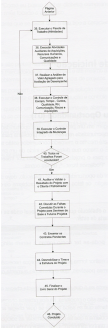
\includegraphics[heigth = \textheight]{figs/fig1.png}
   \caption{Fluxograma}
  \end{figure}
\end{frame}

\begin{frame}
 \frametitle{GRUPO DE PROCESSOS (“FASE”) – \small{EXECUÇÃO, MONITORAMENTO E ENCERRAMENTO}}
  \begin{figure}
   \centering
   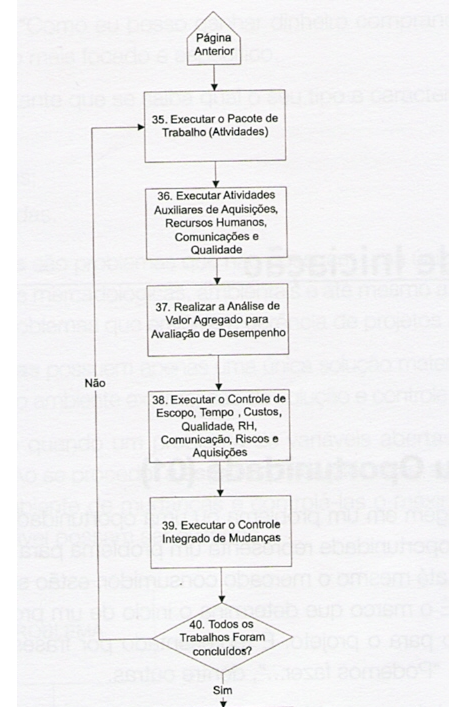
\includegraphics[width = 0.5\textwidth]{figs/fig2.png}
   \caption{Fluxograma}
  \end{figure}
\end{frame}

\begin{frame}
 \frametitle{GRUPO DE PROCESSOS (“FASE”) – \small{EXECUÇÃO, MONITORAMENTO E ENCERRAMENTO}}
  \begin{figure}
   \centering
   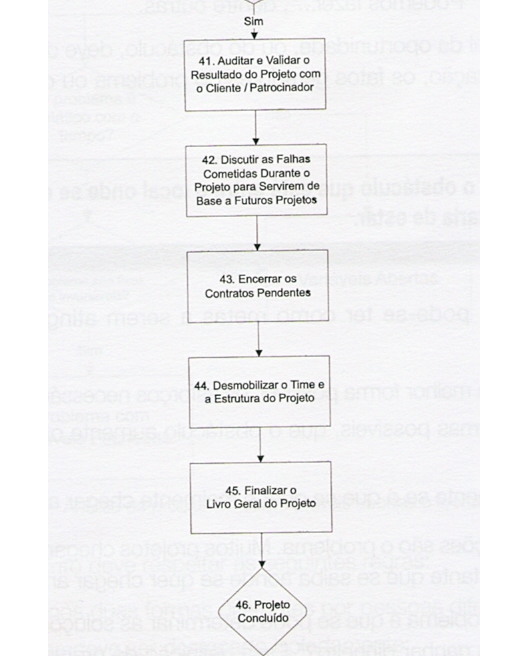
\includegraphics[width = 0.5\textwidth]{figs/fig3.png}
   \caption{Fluxograma}
  \end{figure}
\end{frame}

\begin{frame}
 \frametitle{GRUPO DE PROCESSOS (“FASE”) – \small{EXECUÇÃO, MONITORAMENTO E ENCERRAMENTO}}
  \begin{figure}
   \centering
   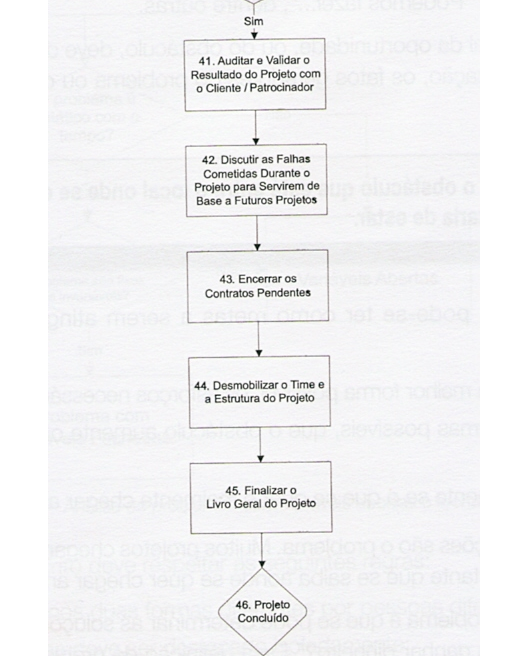
\includegraphics[width = 0.5\textwidth]{figs/fig4.png}
   \caption{Fluxograma}
  \end{figure}
\end{frame}

\section{Executar o Pacote de Trabalho}
\begin{frame}
 \frametitle{GRUPO DE PROCESSOS (“FASE”) – \small{EXECUÇÃO, MONITORAMENTO E ENCERRAMENTO}}
 35 – Executar o Pacote de Trabalho
\begin{block}{}
 A execução dos pacotes de trabalho materializa todo o planejamento do projeto e, portanto, todas as falhas cometidas com etapas anteriores ficam evidentes durante a execução.
\end{block}
\begin{itemize}
 \item A execução é feita através da realização dos pacotes de trabalho
 \item O pacote de trabalho é considerado concluído quando ocorre  a entrega
\end{itemize}
\end{frame}

\begin{frame}
 \frametitle{GRUPO DE PROCESSOS (“FASE”) – \small{EXECUÇÃO, MONITORAMENTO E ENCERRAMENTO}}
 35 – Executar o Pacote de Trabalho
\begin{block}{}
 A execução dos pacotes de trabalho materializa todo o planejamento do projeto e, portanto, todas as falhas cometidas com etapas anteriores ficam evidentes durante a execução
\end{block}
\begin{itemize}
 \item A entrega é qualquer resultado do trabalho que pode ser facilmente medido pelo projeto:
 \begin{enumerate}
  \item facilmente mensurável
  \item tangível pelos executantes
  \item conclusão identificável de maneira simples e direta
 \end{enumerate}
\end{itemize}
\end{frame}

\section{Aquisições, Recursos Humanos, Comunicações e Qualidade}
\begin{frame}
 \frametitle{GRUPO DE PROCESSOS (“FASE”) – \small{EXECUÇÃO, MONITORAMENTO E ENCERRAMENTO}}
 36 – Executar Atividades Auxiliares: Aquisições, Recursos Humanos, Comunicações e Qualidade
\begin{itemize}
 \item Para garantir que os processos de controle e replanejamento sejam eficazes, deve-se:
 \begin{itemize}
  \item Comunicações
  \begin{enumerate}
   \item Distribuir informações no prazo e profundidade desejada
    \item Gerenciar expectativas
  \end{enumerate}
  \item Recursos Humanos
  \begin{enumerate}
   \item 75\% dos processos de RH são executados nesta etapa
    \item Mobilizar equipe
    \item Desenvolver o time
    \item Políticas de premiação por resultados
    \item Gerenciar a equipe
  \end{enumerate}
 \end{itemize}
\end{itemize}
\end{frame}

\begin{frame}
 \frametitle{GRUPO DE PROCESSOS (“FASE”) – \small{EXECUÇÃO, MONITORAMENTO E ENCERRAMENTO}}
 36 – Executar Atividades Auxiliares: Aquisições, Recursos Humanos, Comunicações e Qualidade
\begin{itemize}
 \item Para garantir que os processos de controle e replanejamento sejam eficazes, deve-se:
 \begin{itemize}
  \item Qualidade
  \begin{enumerate}
   \item Garantir que os resultados do projeto estejam de acordo com os padrões de qualidade definidos
   \item Identificar e avaliar as causas de resultados insatisfatórios e eliminá-los
  \end{enumerate}
  \item Aquisições
  \begin{enumerate}
   \item Solicitação de respostas dos fornecedores
    \item Escolher fornecedores
  \end{enumerate}
 \end{itemize}
\end{itemize}
\end{frame}

\section{Realizar a Análise de Valor Agregad}
\begin{frame}
 \frametitle{GRUPO DE PROCESSOS (“FASE”) – \small{EXECUÇÃO, MONITORAMENTO E ENCERRAMENTO}}
 37 – Realizar a Análise de Valor Agregado para Avaliação de Desempenho
\begin{itemize}
 \item Existem várias formas de se avaliar o desempenho de um projeto: variâncias e tendências
  \item Porém, a análise de valor agregado é uma das mais precisas e poderosas técnicas disponíveis
 \end{itemize}
   \begin{figure}
   \centering
   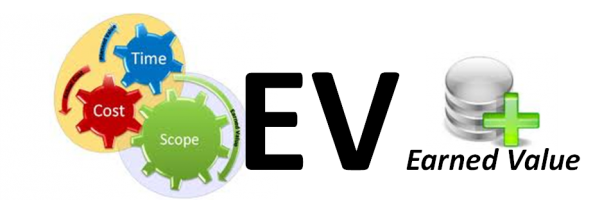
\includegraphics[width = 0.6\textwidth]{figs/fig5.png}
  \end{figure}
\end{frame}

\begin{frame}
 \frametitle{GRUPO DE PROCESSOS (“FASE”) – \small{EXECUÇÃO, MONITORAMENTO E ENCERRAMENTO}}
 37 – Realizar a Análise de Valor Agregado para Avaliação de Desempenho
 \begin{block}{}
  A análise de valor agregado(Earned Value Analysis) é a responsável pelo acompanhamento financeiro de todo o  projeto. Seu objetivo é detalhar os custos do projeto de 
  forma a acompanhar com precisão as evoluções dos custos
 \end{block}
\begin{itemize}
 \item O valor agregado tem foco na relação entre os custos reais consumidos e o trabalho realizado no projeto
  \item Funciona com um tipo de alarme.
  \item Suporte a análise de desempenho.
 \end{itemize}
 \end{frame}
 
 \begin{frame}
 \frametitle{GRUPO DE PROCESSOS (“FASE”) – \small{EXECUÇÃO, MONITORAMENTO E ENCERRAMENTO}}
 37 – Realizar a Análise de Valor Agregado para Avaliação de Desempenho
 
\begin{itemize}
 \item BCWS ou COTA (custo orçado do trabalho agendado)
  \begin{enumerate}
   \item Valor que indica a parcela do orçamento que deveria ser gasta, considerando o custo na linha de base
   \item É calculado como os custos de linha de base divididos e acumulados até a data de referência
   \item Proveniente do orçamento
   \item O PMI utiliza a sigla PV (planned value)
  \end{enumerate}
 \end{itemize}
 \end{frame}
 
\begin{frame}
 \frametitle{GRUPO DE PROCESSOS (“FASE”) –\small{EXECUÇÃO, MONITORAMENTO E ENCERRAMENTO}}
37 – Realizar a Análise de Valor Agregado para Avaliação de Desempenho – Orçamento, Custos Reais e VA
\begin{itemize}
 \item ACWP ou CRTR (custo real do trabalho realizado)
 \begin{itemize}
  \item Mostra os custos reais incidentes para o trabalho já realizado por um recurso ou atividade, até a data de referência
  \item O PMI utiliza a sigla AC (actual cost)
 \end{itemize}
 \end{itemize}
\end{frame}

\begin{frame}
 \frametitle{GRUPO DE PROCESSOS (“FASE”) –\small{EXECUÇÃO, MONITORAMENTO E ENCERRAMENTO}}
37 – Realizar a Análise de Valor Agregado para Avaliação de Desempenho – Orçamento, Custos Reais e VA
\begin{itemize}
 \item BCWP ou COTR (custo orçado do trabalho realizado)
 \begin{itemize}
  \item Valor que indica a parcela do orçamento que deveria ser gasta, considerando o trabalho realizado até o momento e o custo na linha de base
   \item É calculado como o percentual da atividade realizada multiplicada pelo seu orçamento
    \item \textbf{Denominado de Valor Agregado}
    \item O PMI utiliza a sigla EV(earned value)
 \end{itemize}
 \end{itemize}
\end{frame}

\begin{frame}
 \frametitle{GRUPO DE PROCESSOS (“FASE”) – \small{EXECUÇÃO, MONITORAMENTO E ENCERRAMENTO}}
 37 – Realizar a Análise de Valor Agregado para Avaliação de Desempenho – Orçamento, Custos Reais e VA
   \begin{figure}
   \centering
   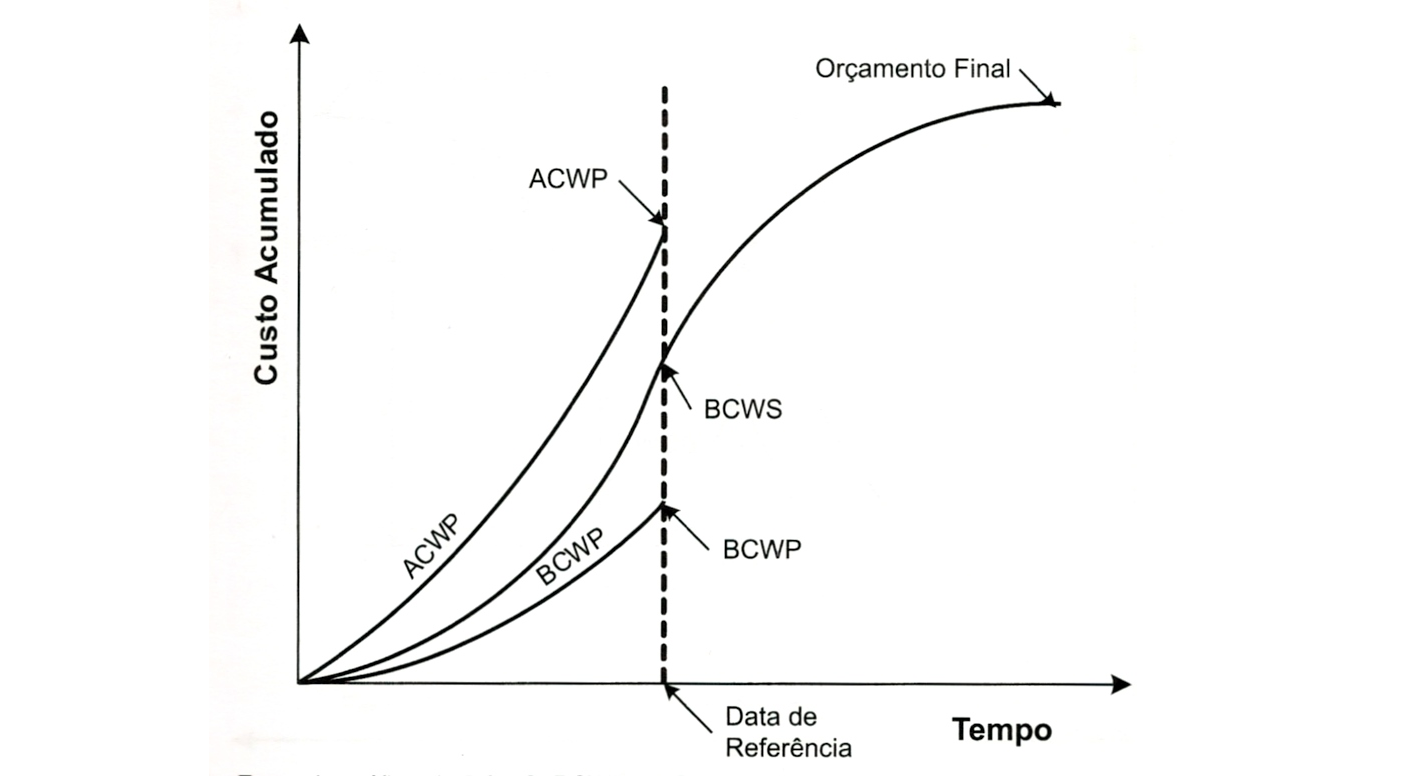
\includegraphics[width = 0.9\textwidth]{figs/fig6.png}
  \end{figure}
\end{frame}

\begin{frame}
 \frametitle{GRUPO DE PROCESSOS (“FASE”) –\small{EXECUÇÃO, MONITORAMENTO E ENCERRAMENTO}}
37 – Realizar a Análise de Valor Agregado para Avaliação de Desempenho – Análises de Variações de Custo e Prazo
\begin{itemize}
 \item CV ou VC (variação do custo)
 \begin{equation}
  CV = BCWP - ACWP
 \end{equation}
 \begin{itemize}
  \item Se CV $>$ 0, o custo do trabalho agregado estará aquém do valor realmente gasto(custo real)
  \item Se CV $<$ 0, houve valor agregado inferior ao que se gastou no trabalho
  \item Mantendo a tendência negativa, significa que o projeto tem grande probabilidade de ser concluído com gasto superior ao orçado
 \end{itemize}
 \end{itemize}
\end{frame}

\begin{frame}
 \frametitle{GRUPO DE PROCESSOS (“FASE”) –\small{EXECUÇÃO, MONITORAMENTO E ENCERRAMENTO}}
37 – Realizar a Análise de Valor Agregado para Avaliação de Desempenho – Análises de Variações de Custo e Prazo
\begin{itemize}
 \item SV ou VP (variação de prazos)
 \begin{equation}
 SV = BCWP - BCWS
 \end{equation}
 \begin{itemize}
  \item Diferença em termos de custo
  \item Se SV $>$ 0, o projeto estará adiantado
  \item Se SV $<$ 0, o projeto estará atrasado
  \item Traduzido pelo PMI como VP ou variação de prazos
 \end{itemize}
 \end{itemize}
\end{frame}

\begin{frame}
 \frametitle{GRUPO DE PROCESSOS (“FASE”) –\small{EXECUÇÃO, MONITORAMENTO E ENCERRAMENTO}}
37 – Realizar a Análise de Valor Agregado para Avaliação de Desempenho – Análises de Variações de Custo e Prazo
\begin{itemize}
 \item TV ou VT (variação de tempo)
 \begin{itemize}
  \item Diferença em termos de tempo
  \item Projeção da curva BCWS e BCWP, encontrando a data em que se agrega valor
  \item A diferença entre a data de referência e a data em que se agrega valor representa o atraso ou adiantamento
 \end{itemize}
 \end{itemize}
\end{frame}

\begin{frame}
 \frametitle{GRUPO DE PROCESSOS (“FASE”) – \small{EXECUÇÃO, MONITORAMENTO E ENCERRAMENTO}}
 37 – Realizar a Análise de Valor Agregado para Avaliação de Desempenho – Análises de Variações de Custo e Prazo
   \begin{figure}
   \centering
   
\includegraphics[width = 0.9\textwidth]{figs/fig7.png}
  \end{figure}
\end{frame}

\begin{frame}
 \frametitle{GRUPO DE PROCESSOS (“FASE”) –\small{EXECUÇÃO, MONITORAMENTO E ENCERRAMENTO}}
37 – Realizar a Análise de Valor Agregado para Avaliação de Desempenho – Índices de Desempenho
\begin{itemize}
 \item SPI ou IDP (índice de desempenho de prazos)
 \begin{equation}
  SPI = \frac{BCWP}{BCWS}
 \end{equation}
 \begin{itemize}
  \item Se SPI $<$ 1, o projeto está atrasado
  \item Se SPI $>$ 1, o projeto está adiantado
  \item Se SPI $=$ 1, o projeto está exatamente no prazo
  \item Mostra a taxa de conversão do valor previsto em valor agregado
 \end{itemize}
 \end{itemize}
\end{frame}

\begin{frame}
 \frametitle{GRUPO DE PROCESSOS (“FASE”) –\small{EXECUÇÃO, MONITORAMENTO E ENCERRAMENTO}}
37 – Realizar a Análise de Valor Agregado para Avaliação de Desempenho – Índices de Desempenho
\begin{itemize}
 \item CPI ou IDC (índice de desempenho de custos)
 \begin{equation}
  CPI = \frac{BCWP}{ACWP}
 \end{equation}
 \begin{itemize}
  \item Se CPI $<$ 1, o projeto está gastando mais do que o previsto
  \item Se CPI $>$ 1, o projeto está custando abaixo do orçamento
  \item Se CPI $=$ 1, o projeto está exatamente no orçamento
  \item Mostra a taxa de conversão entre os valores gastos e os valores agregados no projeto
 \end{itemize}
 \end{itemize}
\end{frame}

\begin{frame}
 \frametitle{GRUPO DE PROCESSOS (“FASE”) – \small{EXECUÇÃO, MONITORAMENTO E ENCERRAMENTO}}
 37 – Realizar a Análise de Valor Agregado para Avaliação de Desempenho –  Índices de Desempenho
   \begin{figure}
   \centering
   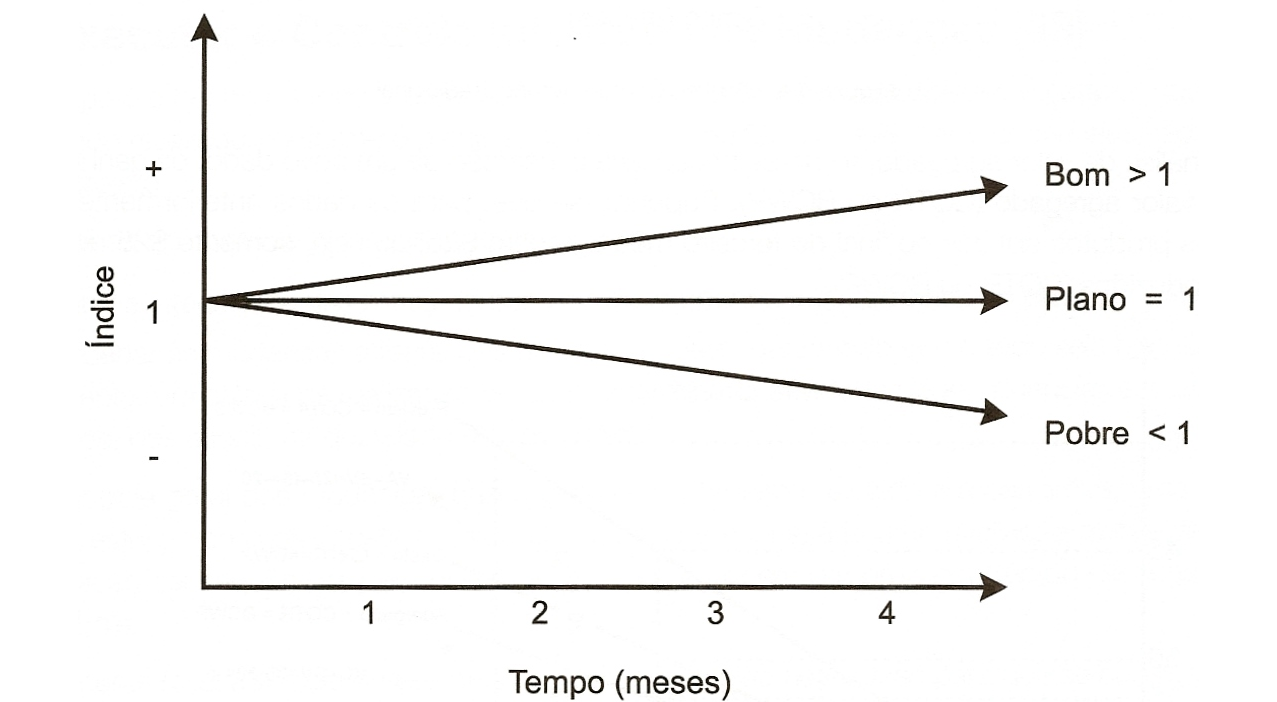
\includegraphics[width = 0.9\textwidth]{figs/fig8.png}
  \end{figure}
\end{frame}


\begin{frame}
 \frametitle{GRUPO DE PROCESSOS (“FASE”) – \small{EXECUÇÃO, MONITORAMENTO E ENCERRAMENTO}}
 37 – Realizar a Análise de Valor Agregado para Avaliação de Desempenho – EXEMPLO
  \begin{itemize}
   \item Tem-se um projeto que custa $R\$60,00$ e tem $4$ meses de prazo para a execução.
   \item Supondo que o gasto de capital seja linear, tem-se um consumo de $R\$15,00$ (COTA ou BCWS)/mês
    \item No final do terceiro mês, o gerente do projeto calcula os gastos do projeto e chega a um total de $R\$30,00$ (CRTR ou ACWP)
  \end{itemize}
\end{frame}

\begin{frame}
 \frametitle{GRUPO DE PROCESSOS (“FASE”) – \small{EXECUÇÃO, MONITORAMENTO E ENCERRAMENTO}}
 37 – Realizar a Análise de Valor Agregado para Avaliação de Desempenho – EXEMPLO
  \begin{itemize}
   \item O projeto economizou, certo?
  \end{itemize}
  \begin{figure}
   \centering
   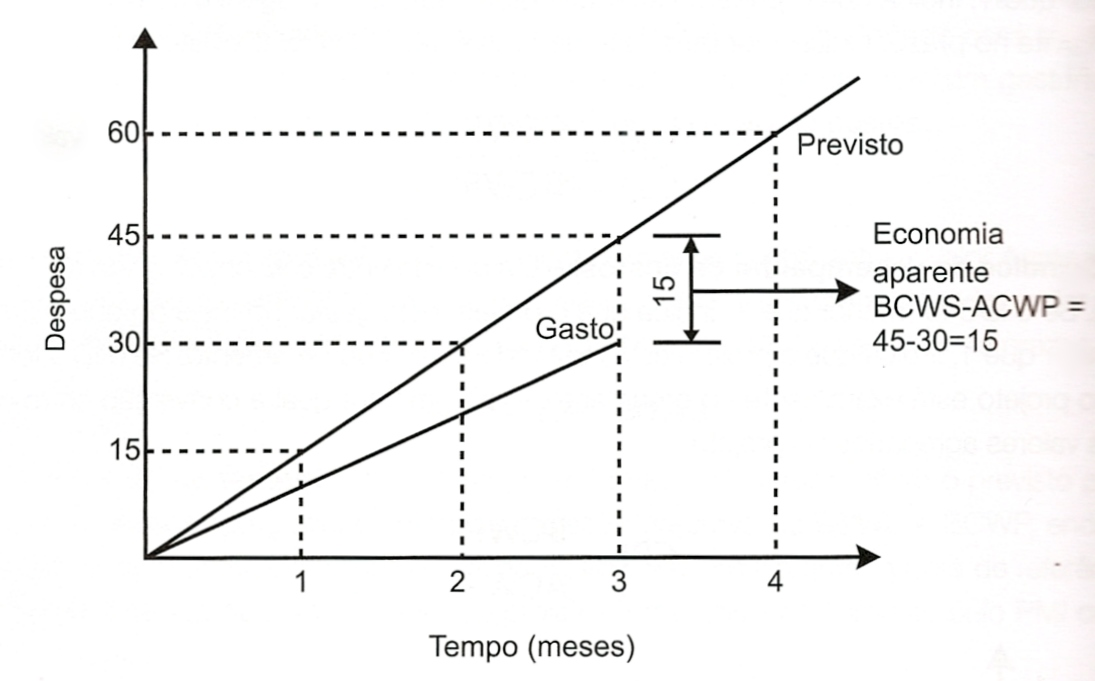
\includegraphics[width = 0.9\textwidth]{figs/fig9.png}
  \end{figure}
\end{frame}

\begin{frame}
 \frametitle{GRUPO DE PROCESSOS (“FASE”) – \small{EXECUÇÃO, MONITORAMENTO E ENCERRAMENTO}}
 37 – Realizar a Análise de Valor Agregado para Avaliação de Desempenho – EXEMPLO
  \begin{itemize}
   \item Ao utilizar a técnica EVA, temos necessidade de analisar os ganhos físicos (COTR ou BCWP)
  \item Supondo que, para os dados anteriormente mencionados, os produtos obtidos no final do terceiro mês agregam $R\$25$
  \end{itemize}
\end{frame}

\begin{frame}
 \frametitle{GRUPO DE PROCESSOS (“FASE”) – \small{EXECUÇÃO, MONITORAMENTO E ENCERRAMENTO}}
 37 – Realizar a Análise de Valor Agregado para Avaliação de Desempenho – EXEMPLO
  \begin{figure}
   \centering
   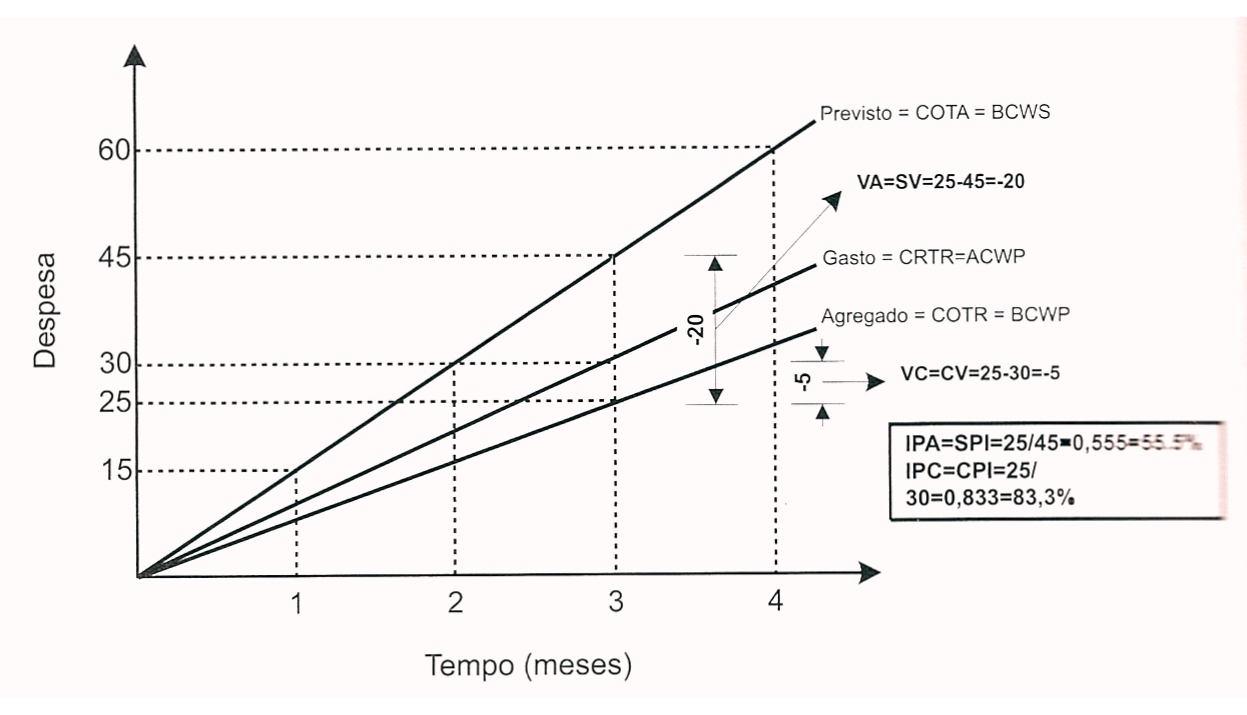
\includegraphics[width = 0.9\textwidth]{figs/fig10.png}
  \end{figure}
\end{frame}


\begin{frame}
 \frametitle{GRUPO DE PROCESSOS (“FASE”) – \small{EXECUÇÃO, MONITORAMENTO E ENCERRAMENTO}}
 37 – Realizar a Análise de Valor Agregado para Avaliação de Desempenho – EXEMPLO (Conclusões/Análises)
  \begin{itemize}
   \item Projeto está atrasado, uma vez que foram agregados apenas $R\$25$ dos $R\$45$ previstos
    \item Está abaixo do planejado em  $R\$20$
    \item O projeto consumiu $R\$30$ para agregar apenas $R\$25$
    \item Além do atraso nos prazos, tem-se aumento nos custos em $R\$5$, 
    \item SPI é de 0,555 (55\%), o que significa, que apenas 55\% do tempo gasto está sendo transformado em resultados e 44,5\% está sendo desperdiçado
    \item CPI é de 0,833(83\%), o que significa que 83,3\% do dinheiro gasto foi convertido em resultados e 16,7\% do dinheiro está sendo desperdiçado
  \end{itemize}
\end{frame}

\begin{frame}
 \frametitle{GRUPO DE PROCESSOS (“FASE”) – \small{EXECUÇÃO, MONITORAMENTO E ENCERRAMENTO}}
 37 – Realizar a Análise de Valor Agregado para Avaliação de Desempenho – Considerações Finais
  \begin{itemize}
   \item O GP deve monitorar a baseline de custos para identificar variações do planejamento original
    \item Medidas de performance devem ser utilizadas como auxílio na identificação dos desvios e no fornecimento de informações aos stakeholders
    \item É importante entender as causas das variações de custo e tomar as medidas corretivas
  \end{itemize}
\end{frame}

\section{Auditar e Validar o Resultado do Projeto }

\begin{frame}
 \frametitle{GRUPO DE PROCESSOS (“FASE”) – \small{EXECUÇÃO, MONITORAMENTO E ENCERRAMENTO}}
 41 – Auditar e Validar o Resultado do Projeto com o Cliente/Patrocinador
 \begin{block}{}
  O objetivo é avaliar o resultado do projeto junto ao cliente ou patrocinador para obter o aceite
 \end{block}
  \begin{itemize}
   \item Em engenharia de software isso equivale a homologação feita pelo usuário, por meio do uso, ao longo de um tempo, com as devidas correções terem sido procedidas
    \item Teste beta, aceitação, release candidate, release final...
    \item Em outros projetos existe um processo mais formal de auditoria, como forma de dar o aceite
  \end{itemize}
\end{frame}


\begin{frame}
 \frametitle{EXERCÍCIO}
  \begin{itemize}
   \item Calcule o valor agregado no projeto de vocês, apresentando os índices de desempenho
  \end{itemize}
\end{frame}


\end{document}
